\documentclass{article}
\usepackage[utf8]{inputenc}

%additional usepackages
\usepackage{amsmath}
\usepackage{eufrak}
\usepackage{tikz}
\usepackage{ amssymb }
\usepackage{import}
\usepackage[ruled,vlined]{algorithm2e}
\usepackage{booktabs}
\usepackage[capposition=top]{floatrow}
\usepackage{scrextend}
\usepackage{csquotes}
\usepackage{graphicx}
\usepackage{pdfpages}

\usepackage{caption}
\usepackage{subcaption}

% bibliography
\usepackage[backend=biber, citestyle=authoryear]{biblatex}
\addbibresource{speciale.bib}

% functions

\newcommand{\quickwordcount}[1]{%
  \immediate\write18{texcount -1 -sum -merge -q #1.tex output.bbl > #1-words.sum }%
  \input{#1-words.sum}%
}

\newcommand{\quickcharcount}[1]{%
  \immediate\write18{texcount -1 -sum -merge -char -q #1.tex output.bbl > #1-chars.sum }%
  \input{#1-chars.sum}(not including spaces)%
}


%%%% INDEPDENT SIGN %%%%

\makeatletter
% Taken from http://ctan.org/pkg/centernot
\newcommand*{\centernot}{%
  \mathpalette\@centernot
}
\def\@centernot#1#2{%
  \mathrel{%
    \rlap{%
      \settowidth\dimen@{$\m@th#1{#2}$}%
      \kern.5\dimen@
      \settowidth\dimen@{$\m@th#1=$}%
      \kern-.5\dimen@
      $\m@th#1\not$%
    }%
    {#2}%
  }%
}
\makeatother

\newcommand{\independent}{\perp\mkern-9.5mu\perp}
\newcommand{\notindependent}{\centernot{\independent}}

\newcommand{\E}{\mathbb{E}}
\newcommand{\N}{\mathbb{N}}
\newcommand{\ndist}{\mathcal{N}}
\newcommand{\std}{\mathbf{std}}
\newcommand{\R}{\mathbb{R}}
\newcommand{\lra}{\Leftrightarrow}

\newcommand{\Loss}{\mathcal{L}}
\newcommand{\loss}{\mathcal{l}}

\newcommand{\la}{\leftarrow}
\newcommand{\ra}{\rightarrow}

\newcommand{\ones}{\mathbf{1}}

\newcommand{\statespace}{\mathcal{S}}
\newcommand{\actionspace}{\mathcal{A}}

\DeclareMathOperator*{\argmax}{arg\,max}
\DeclareMathOperator*{\argmin}{arg\,min}

% paranthesis

\newcommand{\lp}{\left(}
\newcommand{\rp}{\right)}
\newcommand{\lsp}{\left[}
\newcommand{\rsp}{\right]}
\newcommand{\lcp}{\left\{}
\newcommand{\rcp}{\right\}}

% Margins and paragraph indent etc (layout)

\setlength{\parindent}{0em}
\setlength{\parskip}{0.25cm}
\usepackage[margin=1.05in]{geometry}


% About Data
\title{\input{name}}
\author{Jeppe Søndergaard Johansen (pcv439)}
\date{May 2020}

\makeindex


\begin{document}



\includepdf[pages={1}]{frontpage/frontpage.pdf}


\maketitle

Number of characters: \quickcharcount{main}. Maximum is (144.000)

Number of spaces: \quickwordcount{main}

%\begin{abstract}
This paper investigates reinforcement learning as a solution method for dynamic models. A discrete time, finite horizon, discrete choice model of female labour supply and fertility is formulated, and the model is solved using value function iteration and two reinforcement learning methods, namely deep Q-learning and double deep Q-learning. After estimating the model using method of simulated moments, and finding the simple model inadequate to describe data from Statistic Denmark, the model is extended. The extension consists of 14 + 1 states. The extended model is solved only using double deep Q-learning and estimated using simulated method of moments. The results of the extended model convincingly matches data from Statistics Denmark and contemporary findings by \textcite{kleven_children_2019}. I conclude that the field of economics should further investigate reinforcement learning, as it allows solving dynamic models with high dimensional state space.
\end{abstract}


\pagebreak

\tableofcontents

\pagebreak

\section{Introduction} 

The last 10 years have lead to numerous breakthroughs within the field of machine learning, among them especially the subfield of reinforcement learning has experienced great leaps. In 2013 the company DeepMind achieved super human performance in various Atari games \parencite{mnih_playing_2013}. In 2018 the same company beat professional human players in the board game Go, a feat which was not deemed possible in a foreseeable future \parencite{silver_general_2018}, and as late as 2019 DeepMind showed that an reinforcement learning agent was able to play the game of Star Craft 2 on the same level as the best human players \parencite{vinyals_grandmaster_2019}. All the games mentioned can be considered dynamical models. Dynamic models play a central role within the field of economics. The results imply a new way of solving dynamic economic models using reinforcement learning.

Dynamical models usually involve agents that take sequential actions, trying to maximize the cumulative utility from these actions. This class of economic models conform to a set of properties economists like: They have a micro foundation - agents are utility maximizing. They model time, allowing for agents to foresee the future, and act in accordance to their expectations. Some dynamic models can be solved  analytically. This is true for the canonical Ramsey model. However when the scope of the dynamic model grows, different approaches is necessary. Dynamic programming is usually the tool utilized for solving such models.  Even though dynamic programming is a flexible tool it do have its limitations. Solving a model using dynamic programming, requires a limited sized state space, otherwise the computation involved becomes infeasible. In practice this leaves high dimensional dynamic models impossible to solve using contemporary techniques. Deep reinforcement learning allows for solving such models. Because these techniques are relatively novel, they have not yet been introduced into the field of economics. Deep reinforcement learning, does unfortunately not guarantee that the solution converges to the global maximum, but results have shown that learning is possible in hard, high dimensional environments.

This paper uses the aforementioned techniques to investigate the effect of children on female labour supply. Inspired by the model specification of \textcite{francesconi_joint_2002} and \textcite{adda_career_2011} I formulate an discrete time, finite horizon model that models discreet female labour supply and its relationship to fertility. First a simple model is formulated, where women can choose the number of supplied hours, letting fertility be exogenous, with an income process following the Mincer equation of human capital. The husband of the household, is assumed to follow a deterministic path both with regards to number of hours supplied to the labour force, and with the wage rates they receive. Households are assumed to face a budget constraint, that neither allow for borrowing or saving. Utility is assumed to be a function of leisure and consumption, and children are assumed to reduce leisure by mirroring additional work for the woman, that is not financially compensated. Later an extension to the original model is presented with exogenous education combined with a transfer system for women in the education system. Additionally the extension tracks children on an individual level.

Using three different solution methods: value function iteration, deep Q-learning and double deep Q-learning I solve the simple model. I show that one can get comparable performance using deep reinforcement learning compared to using value function iteration solution methods, yielding a new way to solve more complex dynamic models. The parameters of the Mincer equation are calibrated using data from Statistics Denmark . The model is estimated using method of simulated moments, where a simple grid search approach is applied due to fact the optimization problem being one dimensional. The extended model is only solved using double deep Q-learning. Again the model is estimated using method of simulated moments and grid search. The data used for the optimization is from Statistics Denmark.

My two main findings are: 1) Deep reinforcement learning can yield comparable performance to value function iteration solution methods. Considering this allows for solving dynamic models with high dimensional state space, I argue these methods should be explored further in the field of economics. 2) Simulating from the estimated model, I find the initial simple model is not able fit the data, whereas the extended model does fit the data surprisingly well. Both participation rates and average number of supplied hours to labour force, are surprisingly close to what the data from Statistics Denmark suggest. Comparing to  \textcite{kleven_children_2019}, this paper finds results very similar with regards to earnings, participation rate, supplied hours to the labour force and wage rates, when women gives birth to a child.

The paper follows the structure: A literature review is conducted highlighting the main findings and articles of endogenous female labour supply and the effect of children. A model is formulated based on key takeaways from the literature. The parameters of the income process is calibrated using data from Statistics Denmark. Next, I introduce the reader to both reinforcement learning and deep learning. Settling on three different solution methods i solve and estimate the model. I go on to extend the model, and solve it using double deep Q-Learning. I end by comparing the results to contemporary findings, and data from Statistics Denmark.
%\section{Review of Literature}\label{sec:lit_review}

There exists a deep literature on both labour supply and fertility.
As this paper tries to investigate the relationship between women's labour supply and fertility by formulating a dynamic  structural model, the focus will lie on literature that has the same scope. The paper that has been the main inspiration for this paper has been work by \textcite{francesconi_joint_2002}, where he proposes a joint dynamic model of fertility and labour supply of married women. Francesconi formulates a model with a joint decision of fertility and labour supply. Labour supply is considered in his formulation split into three choices: not work, work part-time and work full-time. Furthermore Francesconi proposes a model of human capital accumulation as a function of the labour supply. Additionally he assumes a budget constraint of all income in period $t$ should be consumed in period $t$, and the husbands income and labour supply is modelled to follow an exogenous process.  main findings of the paper is that a clear relationship between earnings ability and preference for work, where women with highest earnings profiles negatively, has the lowest marginal utility of children.

Work has also been done in extending the basic framework proposed by \textcite{francesconi_joint_2002} that models joint decision between fertility and labour supply.  \textcite{adda_career_2011} extends the life cycle model by allowing for savings, and more sophisticated skill atrophy processes,  \textcite{gayle_life-cyle_2006} allows for the participation rate of women to be continuous and \textcite{keane_role_2010} focuses on the marriage market while still allowing for fertility and labour supply being part of the choice set. \textcite{adda_career_2011} suggest that fertility might be falling in developed countries due to significant cost to the careers and future earnings of women. They find that the cost of career interruptions as a consequence of children, is non-linear over the career cycle and has the biggest impact around mid-career. They also find that children has influence on career planning, and the effect of planning to have children, affects the career even before the first child. \textcite{gayle_life-cyle_2006} employ a semi-parametric approach to a panel data setting. Inline with \textcite{francesconi_joint_2002}, \textcite{gayle_life-cyle_2006} finds that having children is less desirable for women on high income trajectories. \textcite{keane_role_2010} finds that differences in skill rental price between black and white women can explain the number of teenage pregnancies, implying again that a relationship between fertility and career trajectories is present.

The joint decision between fertility and labour supply has been investigated before \textcite{francesconi_joint_2002} investigated the problem by proposing a dynamic structural model. Both \textcite{moffitt_estimation_1984} and \textcite{hotz_empirical_1988} utilizes an closed form approach to the problem of fertility and labour supply to estimate an econometric model. \textcite{moffitt_estimation_1984} employs a cross sectional approach and finds that he is able to better fit the bimodal distribution of working hours. While controlling for number of children he finds that more children in general imply women work less. \textcite{hotz_empirical_1988} makes the interessting addition to their model, that fertility is only somewhat a choice of the household, i.e. with some probability the fertility outcome will diverge from the household's expectation. They find that maternal time required for a newborn child is 660 hours per year, decreasing geometrically as the child ages. They also find that children do not reduce a woman's labour supply 1-to-1, rather the time spend on children will be taken from other activities as well.

Looking to the effect of children on labour supply has been investigated by \textcite{angrist_children_1996} finding that, the effect of children on labour supply disappear as the child turns 13. The paper emphasizes the causal link (using IV-estimation) between fertility and labour supply and finds that fertility only have a small effect on the labour supply of women. Considering the effect of children  \textcite{altug_effect_1998} employs a semi-parametric approach to estimating the effect of experience on female labour supple, controlling for children. They find that the impact of children on women's participation rate is ambiguous, but for married women, additional children increases number of hours worked.

\textcite{attanasio_explaining_2008} proposes a structural model, that investigates the extensive margin of women that work, leading them to a formulation where women can either work or not work. Their main addition to their model is letting the households borrow, separating them from \textcite{francesconi_joint_2002} among other earlier studies, that did not allow for such behavior. Human capital is accumulated when women enters the work force. They investigate 3 cohorts (Dole, Clinton and Oprah) as to see the what can account for their different participation rates. Their main finding is that some of the difference can be explained by reduced child-care costs and a reduction in the wage gender gap. A later paper from the same authors \textcite{attanasio_aggregating_2018} they construct a model where they again investigate the participation rate of women. In this formulation they control for family composition and importantly include to "taste-shifters" in the utility function. These are latent variables that us used to explain how the participation rate can change under different circumstances. Their main finding is that heterogeneity of demographics, wealth distribution and the point of the business cycle can explain a lot of the aggregate responses of female labour supply.

\textcite{del_boca_motherhood_2009} investigates uses cross-country European data to investigate the join decision about fertility and labour market participation. They control for personal characteristics as well as childcare system, parental leave system, family allowances as well as part time opportunities. Their main findings include that labour market and social environment do not affect fertility in a significant way. They find however that the institutions that can support women's labour market participation does indeed have impact on the women's labour market participation, especially this effect is the most present in less educated women. These results are somewhat in line with \textcite{haan_can_2009} that investigates the impact of financial incentives on female labour supply by exploiting the variance stemming from the tax and transfer system. They also find that child care subsidies do increase labour supply, however in contrast with \textcite{del_boca_motherhood_2009} they do find that child care subsidies do increase fertility as well.

\textcite{jones_fertility_2008} makes a comparative analysis of the prevalent theories explaining the relationship between fertility and income: whether it is taste or ability that can explain the differences in income. They find that both theories can explain, however the ability hypothesis can only hold under the assumption of a elasticity of substitution between consumption and the number of children. Therefore they conclude that the taste theory is more robust.

\textcite{blundell_female_2016} uses quasi-experiment of the UK tax and welfare reforms of the 1990s and 2000s to investigate women's labour supply. They construct a dynamic model where women can save and accumulate human capital, along with educaiton. They make the women choose education level and their participation rate in the labour market. In contrast with \textcite{francesconi_joint_2002} they do not let fertility be part of the choice space, rather they model it as a random event. They control for demographics etc. They find that labour supply elasticities are generally high (but below 1), except for single mother that seem to have above 1. Another interesting result from the paper is that tax credits do seem to let low-education women into the workforce, however it does not seem to have long term influence on employment or wages for this group. \textcite{eckstein_dynamic_2011} also investigates the discrepancy between lone mothers and married couples by constructing a dynamic life cycle model, their motivation being that while the labour supply of women the last 50 years have had a sharp rising trend, the same cannot be said for unmarried women\footnote{Married women has a gone from 30\% to 60\% employment, where single and divorced women have been at around 70\% employment throughout the sample.}. The authors conclude that the rise in female employment in large part can be explained by the increase in years of schooling and the rise of female wages. They also find that changes in fertility and marital status do not have a big impact. 

Briefly discussing results in a danish context, using Danish data \textcite{kleven_children_2019}. They do find that the long term effects of the arrival of a child reduces earnings by about 20 \%, and the hours worked by 10\% for women, while no effects are notable for men (10 year horizon). The same goes for participation rates which fall about 13 \% and wage rates which falls about 9 \% in the long run for women (10 year horizon). \textcite{jorgensen_life-cycle_2017} investigates the relationship between consumption of non-durable goods and the average number of children, since these follows the same trajectory over the life cycle. He finds that income of the households fall significantly, but in contrast with \textcite{kleven_children_2019} the economic effect is negligible at around 1\% reduction in households with one child compared to households with no children. 

%\section{Model specification}\label{sec:model1}

This paper presents a discrete time, finite horizon, discrete choice model of female labour supply. More specifically I model a household consisting of wife, husband and a zero or more children. The model attempts to address what the effect of children is on the labour supply of women. The model consists of 3 components: 1) An income and human capital component, 2) A fertility process, 3) A leisure and utility component. I model the households from age $Q_{min}=18$ to the terminal age $Q_{max} = 60$. Here it should be noted, that I make the simplifying assumption that the husband and wife has the same age and that the couple is married from age $Q=18$. The age evolves in a deterministic fashion, i.e. the household grows one year older for each step in the model:

\begin{equation}
    Q_{t+1} = Q_t + 1
\end{equation}

For each time step in the model, the agent has to  choose how many hours the woman of the household should supply on a weekly basis. The choice is discreet, and consists of four action values: $H_t \in \{0, 25, 37, 45 \}$. The labour supply of the man in the households is not a choice variable and is therefore considered an exogenous variable.

The households has two income streams, the husband, which is perfectly deterministic, and the wife. The income process of the wife consists of an idiosyncratic component $Z_t$, which follows a random walk:

\begin{equation}
    Z_{t+1} = Z_t + \epsilon_t, \qquad \epsilon_t \sim \ndist (0, \sigma_\epsilon)
\end{equation}

This allows for agents to do display heterogeneity owing to the fact that some unobserved carrier choices will lead to higher wages, even though two otherwise identical agents have been part of the labour force equally long. Since these job characteristics is unobserved, it is assumed to be a random walk. The second component of the income process is a human capital component based on the Mincer equation, as described by \textcite{lemieux_mincer_2006}. That is the the log-transformed wage rate/wage level can be described by the human capital accumulated:

\begin{equation}
    \log \tilde{W}_t = \alpha + \eta_G G_t + \eta_{G^2} G_t^2
\end{equation}

A couple of things to note. In the original formulation by \textcite{lemieux_mincer_2006}, the education level is also included. However, due to the lack of availability of such data I am not able to condition on this. It should also be noted, that the state $G_t$ represents the human capital accumulated of the woman in the household. Finally this equation governs only the wage rage of the women (not of the husband), for whom the wage rate and the supplied number of hours is considered exogenous. The exogenous wage rate of the husband is found using the data set \textbf{LONS50} from Statistics Denmark. And the number of supplied hours for the husband is found using the data set \textbf{LIGEF15}, again supplied by Statistics Denmark. The wage rate of the women will be capped at the minimum wage if the sum of the two components $\tilde{W}_t + Z_t$ is not above the the minimum wage $W_{min} = 120$: 

\begin{equation}
    W_t = \max ( W_{min}, \tilde{W} + Z_t)
\end{equation}

The human capital accumulation process, follows a formulation allowing for depreciation (or skill atrophy):

\begin{equation}
    G_{t+1} = G_t (1-\delta)  + \frac{1}{37} H_t 
\end{equation}

Where 37 being the standard number of hours worked in Denmark. The total income $Y_t$ of the household can now be formulated as:

\begin{equation}
    Y_t = 46 \cdot W_t \cdot H_t + f^M(Q_t)
\end{equation}

Where $f^M$ represents the income from the husband as a function of age. And $46 \cdot W_t \cdot H_t$ is the number of supplied hours pr. week, $H_t$, times the number of weeks, 46, in a year for the average person on the labour market\footnote{Assuming 6 weeks of holiday.} times the wage rate, $W_t$. The income process is a function of the number of supplied working hours, $H_t$, and the states $(Q_t, Z_t, G_t)$. The parameters $\delta, \sigma_\epsilon, \eta_G, \eta_{G^{2}}$ will be calibrated in section \ref{sec:parameter_calibration}.

The second component of the model is the fertility process. The fertility is assumed to be exogenous depending on the age of the woman. This is summed up in the equation below:

\begin{equation}
    K_{t+1} = K_t+ \psi_t, \qquad \psi_t \mid Q_t \sim Bernoulli (p_\psi(Q_t))
\end{equation}

$K_t$ is the number of children in the household. The household is assumed to start with $K_t = 0$ at age $Q=18$. At each step with probability $p_\psi(Q_t)$ the wife gives birth to a child. Allowing for the accumulation of children. The number of children is capped at a maximum of 5 in the model. The probability $p_\psi(Q_t)$ is modelled using data from Statistics Denmark using the data set \textbf{FOD33}. The number of children $K_t$ is part of the state space. 

The third component of the model is the utility and leisure component. The agent is assumed to get utility from leisure, $L_t$, and consumption, $Y_t$. Following \textcite{francesconi_joint_2002} the households are assumed to face a budget constraint such that all income of period $t$ must be consumed period $t$.The utility $U_t$ is given by:

\begin{equation}
    U_t = \beta_L \ln(L_t + 1) + \beta_Y \ln(Y_t + 1)
\end{equation}

Following the formulation of \textcite{adda_career_2011}, dividing the utility into sub-utility functions, where each sub-utility function allows for curvature by specifying a constant relative risk-averse (CRRA) function for each sub-utility. Assuming the special case of $\ln(\cdot)$. The parameters $\beta_L, \beta_Y$ is the individual weighing of the different sub-utilities. Note that for identification I will restrict $\beta_Y= 1$. The total number of hours leisure the agent receives in a year follows: 

\begin{equation}
    L_t = 46 \lp \lp 24 \cdot 7 \rp - \omega \cdot K_t - H_t \rp
\end{equation}

Following \textcite{firestone_estimation_1988}, \textcite{thrane_men_2000} and \textcite{ekert-jaffe_time_2015} I assume that some of the time spent with children can be considered work. The number of hours spent on children each week is captured by $-\omega \cdot K_t$. I let $\omega=3.5$ be the time spent of extra house work pr. child each week. This number is taken from \textcite{ekert-jaffe_time_2015}. The weekly number of hours supplied to the labour market $H_t$ is also subtracted from the total amount of leisure. The number of hours is aggregated to annual level subtracting 6 weeks for holiday. To conclude $\beta_L$ will be a parameter estimated to give the best fit of the model

Summarizing the model; the model contains 4 states: $(G)$ human capital, $(Z)$ the idiosyncratic wage path, $(K)$ the number of children in the household and lastly $(Q)$ age. The action taken in each period $(H)$ represents the number of hours the woman supplies to the labour market on a weekly basis. Other important variables are: $(W)$ the wage rate, $(\tilde{W})$ the human capital dependent wage rate,  $(U)$ the utility and $(L)$ leisure. Formally this imply:

\begin{equation}
    \textbf{State space: }\statespace = \R^{2} \times \{0, 1, 2, 3, 4, 5\} \times \{ 18, 19, \cdots, 60\}
\end{equation}

\begin{equation}
    \textbf{Action space: }\actionspace  = \{0, 15, 25, 37, 45\} 
\end{equation}

\begin{equation}
    \textbf{States: }\{G, Z, K, Q\}, \qquad \textbf{Actions: } \{H\} 
\end{equation}

The model furthermore contains the following parameters: $\alpha, \eta_G, \eta_{G^2}, \delta, \sigma_\epsilon, \beta_L, \beta_Y=1, W_{min}=120, \omega=3.5$. Where the parameters governing the income process $(\alpha, \eta_G, \eta_{G^2}, \delta, \sigma_\epsilon)$ will be calibrated using a simple agent based model, and $\beta_L$ will be estimated using the full model. The recursive formulation of the model is given below:

\begin{align}
    U_t(L_t, Y_t) &= \beta_L \ln(L_t + 1) + \beta_Y \ln(Y_t + 1) \label{eq:utility_v1}\\
    L_t(K_t, H_t) &= 46 \cdot ((24 \cdot 7) - \omega \cdot K_t  - H_t) \label{eq:leissure_v1}\\
    \log \tilde{W}_t (G_t) &= \alpha + \eta_G G_t + \eta_{G^2} G_t^2 \label{eq:salary_tilde_v1}\\
    W_t(\tilde{W}_t, Z_t) &= \max(W_{min} , \tilde{W}_t  + Z_t)  \label{eq:salary_v1}\\
    Y_t(Q_t,H_t, W_t) &= 46 \cdot H_t \cdot W_t + f^M(Q_t) \label{eq:total_salary_v1}\\
\end{align}

Law of motion:

\begin{align}
    Q_{t+1}(Q_t) &= Q_t \label{eq:age_v1}\\
    K_{t+1}(K_t, Q_t)  &= K_{t} + \psi_t, \qquad \psi_t \mid Q_t \sim Bernoulli(p_\psi(Q_t)) \label{eq:fertility_v1} \\
    Z_{t+1}(Z_t) &= Z_t + \epsilon_t, \qquad \epsilon_t \sim \ndist(0, \sigma_\epsilon) \label{eq:idiosyncratic_wage_path_v1}\\
    G_{t+1}(G_t) &= G_t(1 - \delta) + \frac{1}{37} H_t \\
\end{align}



\section{Model - Exogenous Fertility}\label{sec:model1}

\begin{equation}
    \textbf{State space: }\statespace = \R^{2} \times \{0, 1, 2, 3, 4, 5\} \times \{ 18, 19, \cdots, 70\}
\end{equation}

\begin{equation}
    \textbf{Action space: }\actionspace  = 46 \cdot \{0, 15, 25, 37, 45\} 
\end{equation}

\begin{equation}
    \textbf{States: }\{G, Z, K, Q\}, \qquad \textbf{Actions: } \{H\} 
\end{equation}

The model represents the labour supply of married women - and the effect of children. More precisely it models a woman who can accumulate human capital by supplying a desired number of working hours. The woman can with a certain probability in each period give birth to a child, where, the number of children influences the utility. The model presented here has 4 states: $G$ which represents human capital, $Z$ which represents the agents idiosyncratic wage path, $K$ the number of kids owned by the agent and $Q$ which evolves in a deterministic fashion and represents the age of the agent. The action the agent can take in each period is a discrete number of working hours $H$.

\begin{equation}
    \textbf{Variables: }\{S, W, Y, M, U, L\},  \qquad \textbf{Parameters: } \{\beta_K, \beta_L, \beta_Y, p_\psi, \sigma_\epsilon, \delta, \zeta\}
\end{equation}


To elaborate the rest of the model variables: $U$ is the utility. Following the formulation of (Adda, Dustman, Stevens - The Career Cost of Children XXX), dividing the utility into sub-utility functions, where each sub-utility function allows for curvature by specifying a constant relative risk-averse (CRRA) function for each sub-utility. Assuming the special case of $\ln(\cdot)$. The parameters $\beta_K, \beta_L, \beta_YK$ is the individual weighing of the different sub-utilities. Note that for identification I will restrict $\beta_Y= 1$. $W_t$ the wage for given year as function of the supplied working hours and hourly salary $S$. The hourly Salary has three components: the minimum wage: $\zeta=120$, $G_t$ the human capital and at last $Z_t$ the idiosyncratic wage path. I assume that the three parts are additive. $Y_t$ represents the households total earning, where $M_t$ is the earnings of the husband, $W_t$ mentioned above is the salary of the woman. Lastly $M_t$, the husbands wage is assumed to be a deterministic function of age. It is modelled non parametric using data from Danmarks Statistik Bank.

The states of the agent evolves the following way: $Q_t$ evolves deterministcally. $K_t$ evolves by with a certain probability and ekstra children is added to the household. This probability is dependent on the age of the women $Q$. The idiosyncratic wage path of the women follows a random walk. The Human capital accumulates with a constant depreciation rate $\delta$. adding the number of working hours last period.

\begin{align}
    U_t(K_t, L_t, Y_t) &= \beta_K \ln(K_t) + \beta_L \ln(L_t) + \beta_Y \ln(Y_t) \\
    W_t(S_t, H_t) &= S_t \cdot H_t \\
    \log \tilde{S}_t (G_t, Z_t) &= \alpha + \eta_G \log(G_t + 1) + \eta_Z \log (Z_t + 1) \\
    S_t(\tilde{S}_t) &= \max(S_{min} , \tilde{S}_t)  \\
    Y_t(W_t, M_t) &= W_t + f^M(Q_t)\\
\end{align}


Law of Motion.

\begin{align}
    Q_{t+1}(Q_t) &= Q_t \\
    K_{t+1}(K_t, Q_t)  &= K_{t} + \psi_t, \qquad \psi_t \mid Q_t \sim Bernoulli(p_\psi(Q_t)) \\
    \log Z_{t+1}(Z_t) &= \log Z_t + \epsilon_t, \qquad \epsilon_t \sim \ndist(0, \sigma_\epsilon) \\
    G_{t+1}(G_t) &= G_t(1 - \delta) + H_t \\
\end{align}


%\begin{figure}
%    \centering
%    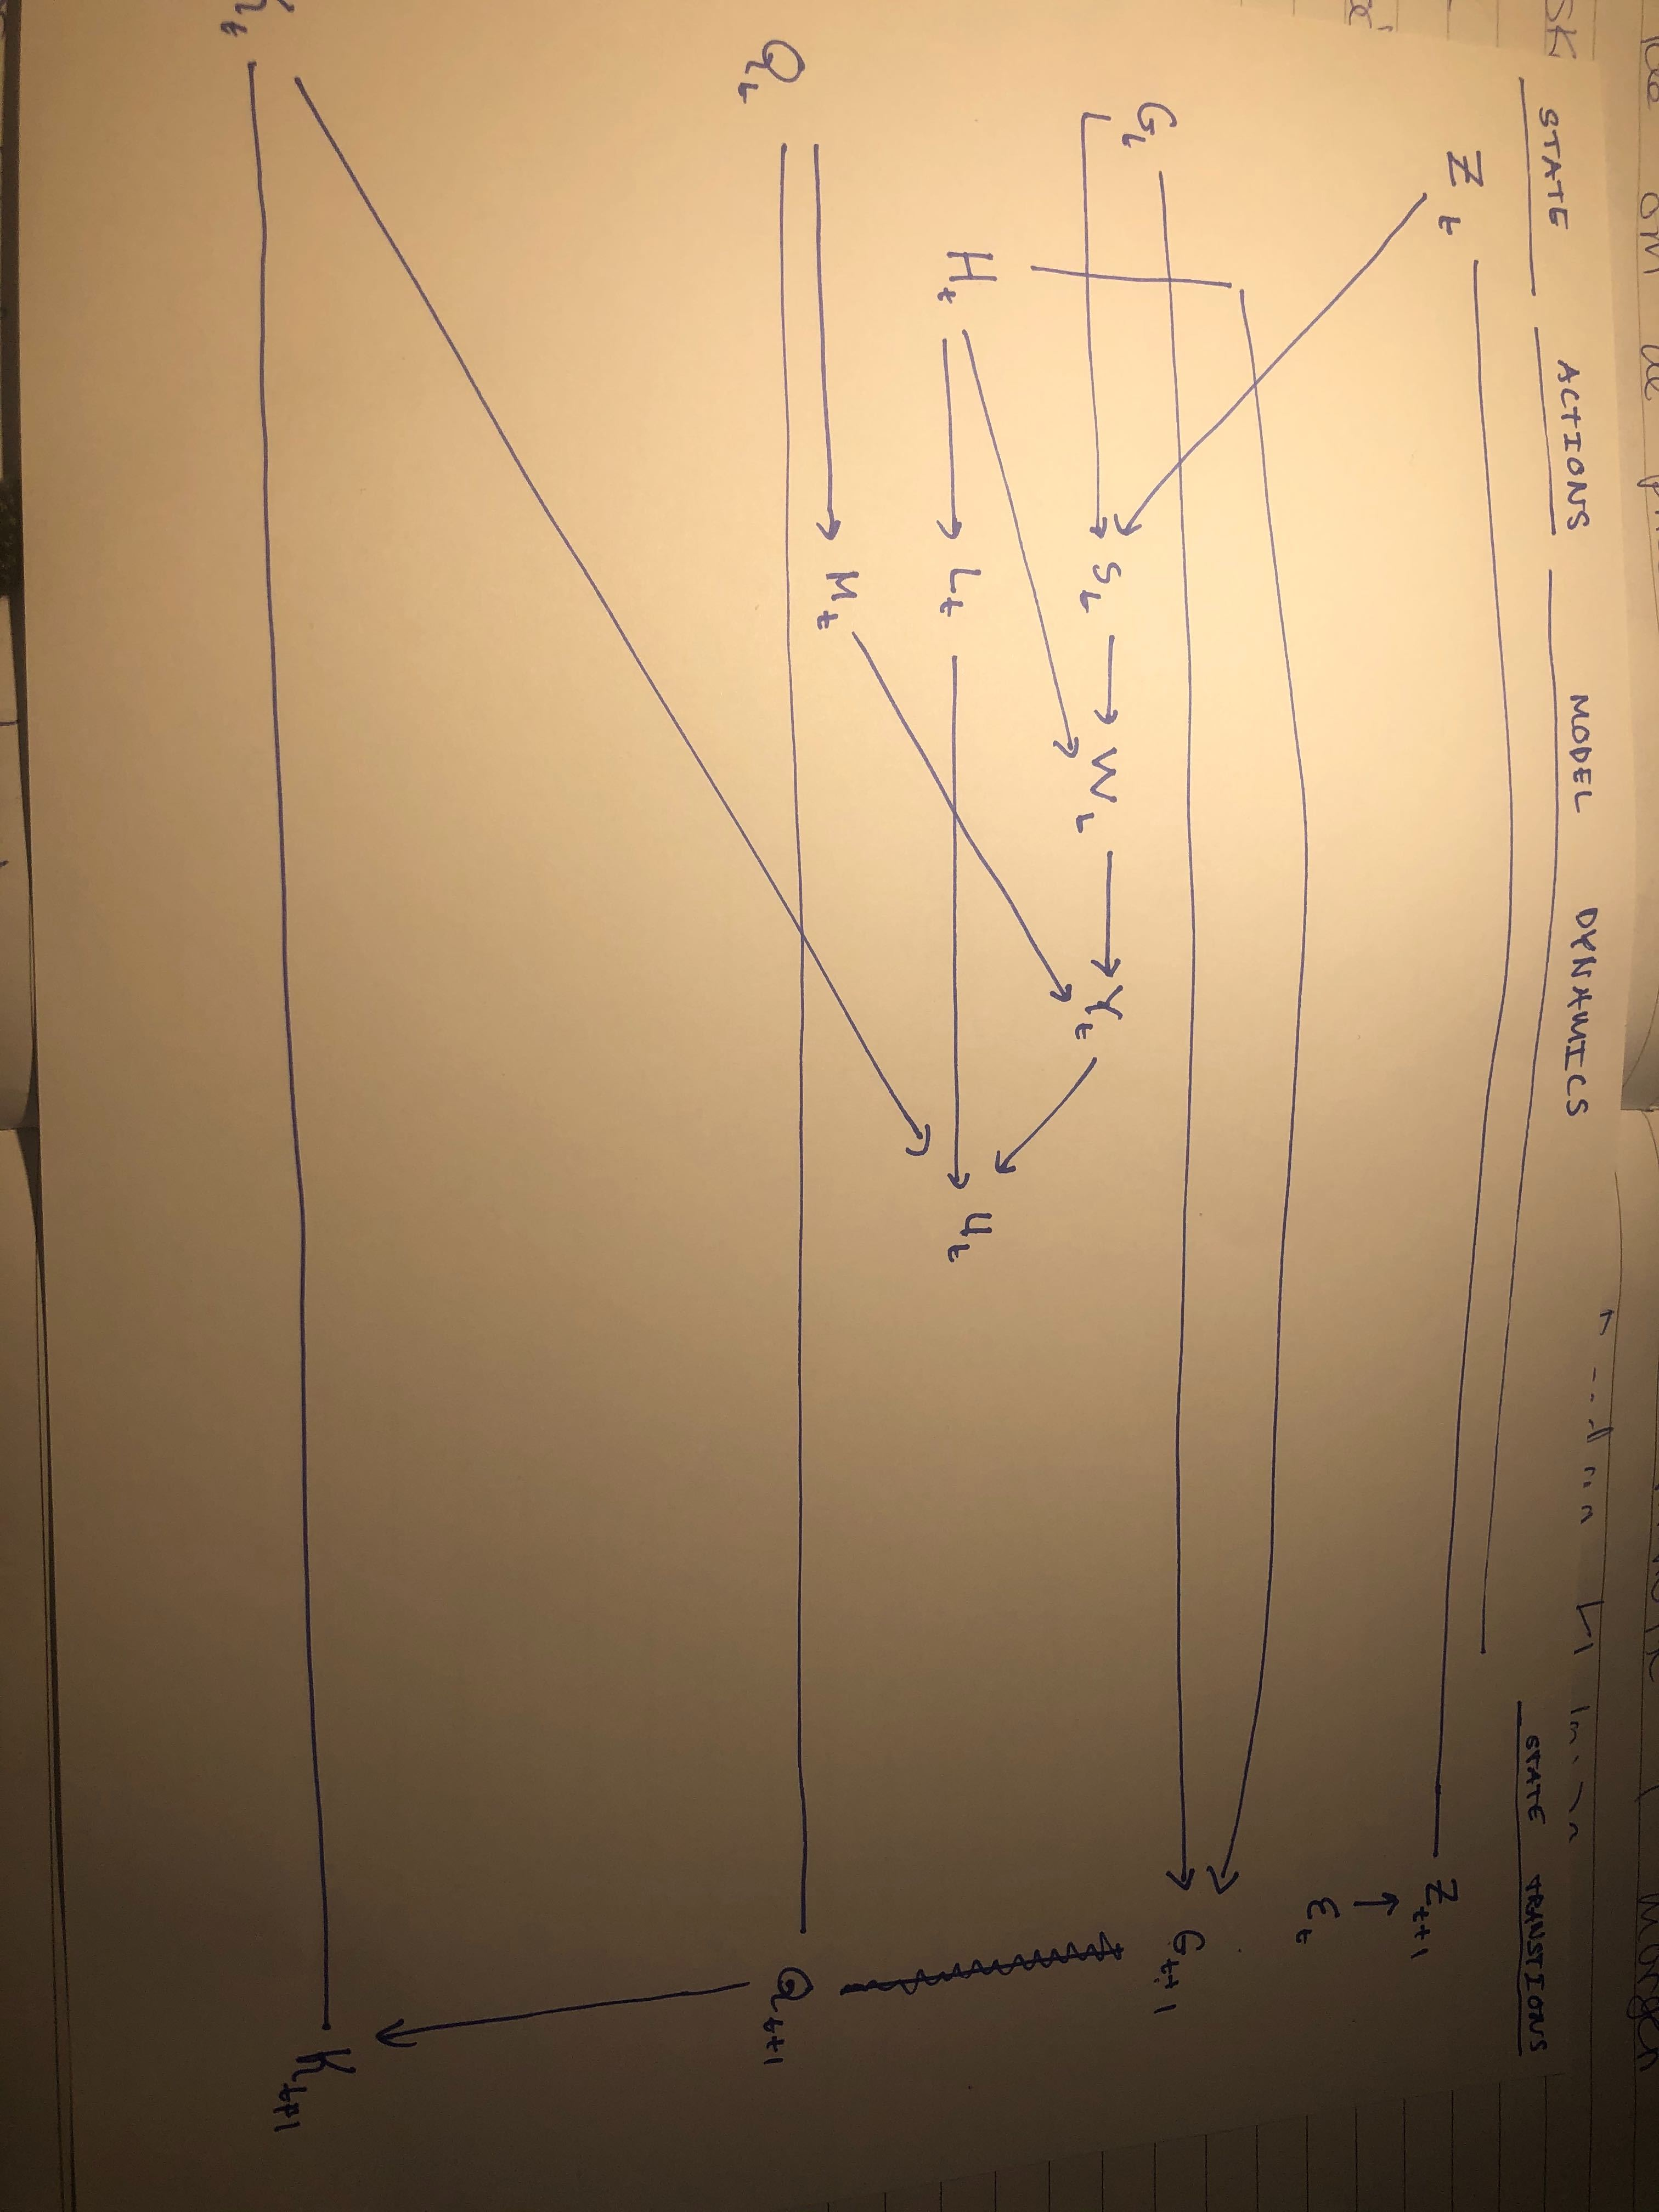
\includegraphics[scale=0.1, angle=90]{figures/modeldynamic_tmp_exogenous.jpg}
%    \caption{Model dynamics - Exogenous (TMP)}
%    \label{fig:tmp_modeldynamics_exogenous}
%\end{figure}

%\section{Model - Endogenous Fertility}

\begin{equation}
    \textbf{State space: }\statespace = \R^{2} \times \{0, 1, 2, 3, 4, 5\} \times \{ 18, 19, \cdots, 70\} \times \{0, 1, 2, 3, 5 \}
\end{equation}

\begin{equation}
    \textbf{Action space: }\actionspace  = \{(0, 0), (0, 1), (46\times15, 0), (46\times25, 0), (46 \times 37, 0), (46 \times 45, 0)\}
\end{equation}

\begin{equation}
    \textbf{States: }\{G, Z, K, Q, A, X\}, \qquad \textbf{Actions: } \{H, F\} 
\end{equation}

The model represents the labour supply of married women - and the effect of children. More precisely it models a woman who can accumulate human capital by supplying a desired number of working hours. The woman can with a certain probability in each period give birth to a child, where, the number of children influences the utility. The model presented here has 4 states: $G$ which represents human capital, $Z$ which represents the agents idiosyncratic wage path, $K$ the number of children living in the household, and $Q$ which evolves in a deterministic fashion and represents the age of the agent. The action the agent can take in each period is a discrete number of working hours $H$. \textbf{$F$ represents the fertility and represents whether or not the household/woman expands the household with an additional child. Note that it is assumed, that if the households conceives a child, the women cannot work in the same period. $A$ is the age of the youngest child (max 5) in the household / or the number of periods since $F=1$. If $K=0 \Rightarrow A=5$. At last $X$ is whether or not the household is able to conceive a child in period $t$}

\begin{equation}
    \textbf{Variables: }\{S, W, Y, M, U, L\},  \qquad \textbf{Parameters: } \{\beta_K, \beta_L, \beta_Y, \beta_A, \sigma_\epsilon, \delta, \zeta, \eta\}
\end{equation}

To elaborate the rest of the variables of the model: $U$ is the utility. Following the formulation of (Adda, Dustman, Stevens - The Career Cost of Children XXX), dividing the utility into sub-utility functions, where each sub-utility function allows for curvature by specifying a constant relative risk-averse (CRRA) function for each sub-utility. Assuming the special case of $\ln(\cdot)$. \textbf{The parameters $\beta_K, \beta_L, \beta_Y$, $\beta_A$ is the individual weighing of the different sub-utilities}. Note that for identification I will restrict $\beta_Y= 1$. $W_t$ the wage for given year as function of the supplied working hours and hourly salary $S$. The hourly Salary has three components: the minimum wage: $\zeta=120$, $G_t$ the human capital and at last $Z_t$ the idiosyncratic wage path. I assume that the three parts are additive. $Y_t$ represents the households total earning, where $M_t$ is the earnings of the husband, $W_t$ mentioned above is the salary of the woman. Lastly $M_t$, the husbands wage is assumed to be a deterministic function of age. It is modelled non parametric using data from Danmarks Statistik Bank.

The states of the agent evolves the following way: $Q_t$ evolves deterministcally. \textbf{$K_t$ evolves by adding the fertility in each period $t$}. The idiosyncratic wage path of the women follows a random walk. The Human capital accumulates with a constant depreciation rate $\delta$ adding the number of working hours last period. \textbf{$A_t$, evolves by taking the max of the age of the age of the youngest child in the household and $\eta=5$. The underlying assumption being at age 5 the parents are indifferent of the age difference between their children. $X_t$ models the probability of the household being able to have a child in the given period. This being stochastic and being dependent on the age of the woman}.

\begin{align}
    U_t(K_t, L_t, Y_t, A_t) &= \beta_K \ln(K_t) + \beta_L \ln(L_t) + \beta_Y \ln(Y_t) + \beta_A \ln(\eta - A_t) \\
    W_t(S_t, H_t) &=S_t \cdot H_t \\
    S_t(Z_t, G_t) &= \min(\zeta, (\zeta + Z_t + G_t))  \\
    Y_t(W_t, M_t) &= W_t + M_t\\
    M_t(Q_t) &= f^M(Q_t) \\
\end{align}


Law of Motion.

\begin{align}
    Q_{t+1}(Q_t) &= Q_t \\
    K_{t+1}(K_t, F_t)  &= K_{t} + X_t \cdot F_{t} \\
    Z_{t+1}(Z_t) &= Z_t + \epsilon_t, \qquad \epsilon_t \sim \ndist(0, \sigma_\epsilon) \\
    G_{t+1}(G_t) &= G_t(1 - \delta) + H_t \\
    A_t(A_t, F_t) &= (1 - F_t) \cdot \max(A_t + 1, \eta)  \\
    X_{t+1}(Q_t) &= \psi_t \qquad \psi_t \sim Bernoulli(p_\psi) \mid Q_t
\end{align}



\section{Deep Learning}
\label{sec:deep_learning}


\subsection{Why machine learning}

Machine learning methods try to model either the joint or the marginal distribution of some covariates and some target. In statistics a model is usually explicitly formulated. A typical example could be linear regression. The covariates is decided on, and transformed such that they fit the desired model. The linear regression will yield a parameter vector which can then be interpreted. And this interpretation is usually the focus - parameter inference. Example: Does an increase in the minimum salary have a negative effect on BNP pr. capita. Machine Learning focuses on prediction. That is, the objective is to predict some target conditional on some covariates. The specific model is not necessarily important. Instead a focus on Out-Of-Sample error is the focus. These predictive methods lend themselves well where causal inference is not needed. Example: What is the expected consumption on a monthly basis by person with a given set of characteristics. When formulating a traditional econometric method, f.x. OLS, there is standard ways to infer if the model is well specified. In machine learning, in general the same asymptotic results regarding regularization of the model is not possible. Usually sample splitting will be used instead. Take a data set, split the data set into two partitions a test set and a training set. First the hyper parameters of the machine learning algorithm is tuned, usually by finding which set of hyper parameters that yield the best performance on the training data. Usually a cross validation procedure is used to find this. The final algorithm is only used on the test data set once yielding the out-of-sample performance. Machine learning methods, as mentioned before usually has associated hyper parameters. These are parameters of the model, which is not fitted by training the data, rather these are specifications of the algorithm before  training the model. Much of machine learning is about finding the right hyper parameters and regularizing the model in an intelligent way \parencite{friedman_elements_2001}. Now why is this paper concerned with ML methods? This is due to the fact, that when estimating the value function, or the policy function, one cannot be sure that this follows a linear function. In fact value functions and policy functions might be highly non-linear, which is where machine learning methods shine. Furthermore what is modelled trying to capture the value function is a conditional expectation: $ \E[Y \mid X=x]$, which can be directly translated into the expected value function for a given state. In this case the causal interpretation of the influence of a specific state on the value function is not of interest, rather it's the accuracy of the expected value function\footnote{Obviously, intelligent agents usually do causal inference on their actions. They might not do a certain action exactly because they have some causal notion of how the environment will evolve conditional on their action.}. Usually deep neural networks has been the usual way to implement reinforcement algorithms, however other machine learning methods can also be used. Deep Learning methods has though they convenient property of online updating of it's weights. In other words, as more data comes in, the neural network can be incrementally fitted to the new data.

\subsection{Deep Neural Networks}

Deep learning (feed forward networks) which is used in this paper is in fact just layered non-linear functions. Figure \ref{fig:feedforwardnetwork} illustrates the architechture of a deep neural network \footnote{Figure found at \url{https://upload.wikimedia.org/wikipedia/commons/thumb/c/c2/MultiLayerNeuralNetworkBigger_english.png/381px-MultiLayerNeuralNetworkBigger_english.png}}.

\begin{figure}[ht]
    \centering
    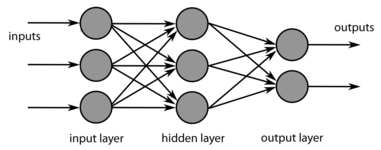
\includegraphics[scale=0.6]{figures/feedforwardnetworkillustration.png}
    \caption{Illustration of feed forward neural network. }
    \label{fig:feedforwardnetwork}
\end{figure}

The network can be described as having an \textit{input layer}, that takes the covariates, $\textbf{x}$. The \textit{hidden layer} makes a transformation, of the previous layer, that also implies that a hidden layer, can be followed by an arbitrary number of other hidden layers. Lastly and \textit{output layer} that maps the representation of the hidden layer into the desired output. For classification that might be a one-hot encoding of the classes, and for regression it might to a single real valued scalar.

As illustrated in figure \ref{fig:feedforwardnetwork}, each layers is broken down into smaller cells. The number of cells in each layer corresponds to the width of the layer. The wider the layer the more flexible representation the given layer is capable of doing. The hidden cells work as mentioned by creating a non-linear transformation of the input from last layer:

\begin{equation}
    z_i^{+} = g(\textbf{z}; \theta) = g(\textbf{w}^T \cdot \textbf{z} + b)
\end{equation}

The output of cell \textit{i} is the real valued scaler $z_i^+$. $g$ is the activation function that maps the input into the output. $\textbf{w}$ is the weights of dot product, $\textbf{z}$ is a vector of the outputs from the last layer, and $b$ is bias or the constant in the activation. In that sense the activation looks like a linear regression squashed through an activation function $g$. Multiple different activations functions has been proposed. Originally the logistic function was prefered, but in later years the rectified linear unit activation function has been popular \parencite{goodfellow_deep_2016}:

\begin{equation}
    \textbf{Rectified Linear Unit: }  \max \lcp 0, \textbf{w}^T \cdot \textbf{z} + b \rcp
\end{equation}

The neural network can in other words be considered a function $f$, that takes an input $\textbf{x}$ and maps it to some output $y$, parametrized by $\theta$, which is a collection of all the weights and biases associated with each individual cell.

\subsection{Stochastic Gradient Descent and Optimization}

The neural network is estimated (or trained) by using stochastic gradient descent. This is possible due to the fact, that the networks can be represented as set of nested functions, such that the chain rule can be applied. The loss function can in other words be differentiated with respect to the parameter vector $\theta$ as shown below:

\begin{equation}\label{eq:loss_function}
    \frac{\partial}{\partial\theta} \Loss (\textbf{X}, \textbf{Y}, \theta) = \frac{\partial}{\partial\theta} \lp \sum \ell_i \rp = \frac{\partial}{\partial\theta} \lp \sum \lp \hat{Y}_i  - Y_i \rp^2 \rp = \frac{\partial}{\partial\theta} \lp \sum \lp f^{\theta}(X_i)  - Y_i \rp^2 \rp
\end{equation}

In equation \eqref{eq:loss_function} the loss function $\Loss$ is assumed be be a mean squared error, in other words a regression problem. The optimization works by minimizing the loss with respect to the parameters $\theta$. In modern neural network architectures it is not unusual that such network has in the excess of a million parameters. Furthermore the objective function of the optimization cannot be assumed to be convex. This implies that analytical solutions for solving deep neural networks is infeasible. Instead gradient descent is used for estimating the parameters of the network. The update rule of the parameters can be described as \parencite{goodfellow_deep_2016}:

\begin{equation}
    \theta \la \theta - \alpha \nabla_{\theta} \Loss(\textbf{X}, \textbf{Y}, \theta)
\end{equation}

So for each step in the algorithm the derivative with of the loss function with respect to the parameters can be calculated, and the parameters can be updated by taking a small step of size $\alpha$ in the direction in parameter space that reduces the loss. Stochastic gradient is a response to the fact that it can be computationally expensive to calculate the gradient for the entire data set in each update step. This is important for deep neural networks, since the training period of a large network, even on optimized hardware, can take a very long time, so any speed up for the training is important. In practice this implies that the training data is split into mini batches usually of size 32 to 128. The optimization is then performed on each of the small batches, taking a small step of size $\alpha$ for each step.




\section{Calibrating the Parameters of the Mincer Equation}


To solve the model some reasonable values for the parameters of the wage process is necessary. The wage process contains the parameters: $(\eta_G, \eta_{G^2}, \delta, \alpha, \sigma_{\epsilon})$. As mentioned in the model specification in section \ref{sec:model1}, the wage process follows the Mincer earnings equation, not accounting for education, and where the idiosyncratic wage path is added linearly to the wage. I assume that the parameters driving the wage process are the same for both men and women, and these can be by calibrated independent of the entire model. This is in part due to computational constraint. \textcite{friedman_elements_2001} argues that calibrating multiple parameters at the same time suffers from the \textit{curse of dimensionality}. Another more important reason is that the wage of the husband in the model is assumed perfectly deterministic, which imply I am not able to calibrate the parameters driving the wage path under the assumption these are the same for men and women in the underlying economy. As mentioned in the model specification, the idiosyncratic wage path is added linearly. This  allows for a two-step calibration of the parameters. First calibrate $(\eta_G, \eta_{G^2}, \delta, \alpha)$ that drives the age and sex specific expected wage rate (referred to as \textit{wage path}). Second the scale of the random walk can be calibrated by $\sigma_\epsilon$ (referred to as \textit{wage variance}). In other words the parameter calibration of the income process is broken into two phases: First calibrating age and sex specific expected wage rate, second calibrating the variance of the wages. It is important to note that this is agent based modelling, where the agent is supplied with a predetermined course of action dependent on the state! 

I calibrate the wage path by using \textbf{LONS50}, a data set from Statistics Denmark (Danmarks Statistik Bank). This data set contains the wage trend for men and women at any given age. The objective is to minimize the squared distance between the empirical wage path and the simulated wage path. The simulated wage path is constructed by simulating from the partial model with given parameters and taking the average. Certain things should be noted about this partial model. The wage path is a function of human capital which again is a function of the choice variable $H$ of the model specified in section \ref{sec:model1}. This obviously makes it problematic to calibrate the parameters. I work around the problem by using the data set \textbf{LIGEF15} containing the number of worked hours for both men and women, which is supplied by Statistics Denmark. These numbers do not take into account people leaving the labour force temporarily, which women are known to do when giving birth. I make the assumption that women leave the work force for 1 year when giving birth to a child. I use the data set \textbf{FOD33} to get fertility rates of women. Again this data is supplied by Statistics Denmark. Formally this can be summed up in the policy described below:

\begin{equation}
    H_t = \begin{cases}
        H^{men}(Q) & \text{if sex=\textit{male}} \\
        H^{women}(Q) & \text{if sex=\textit{female} and birth=\textit{false}} \\
        0 & \text{if sex=\textit{female} and birth=\textit{true} }\\
    \end{cases}    
\end{equation}

The rest of the wage process follows the model described in section \ref{sec:model1}. The minimization problem follows the process:

\begin{equation}
    \text{Cohort Average: } {\tilde{\mu}}_i (C_i) = \frac{1}{\mid C_i \mid} \sum_{\tilde{w}_{n, q} \in C_i} {\tilde{w}_{n, q}}
\end{equation}

\begin{equation}
 (\hat{\eta_G}, \hat{\eta_{G^2}}, \hat{\delta}, \hat{\alpha})   =  \underset{\eta_G, \eta_{G^2}, \delta, \alpha}{\argmin}  \frac{1}{2}\frac{1}{\mid C \mid } \sum_{C_i \in C} \lp\lp \mu_{i}^{men}(C_i)  - \tilde{\mu}_i^{men}(C_i)\rp^2 + \lp \mu_{i}^{women}(C_i)  - \tilde{\mu}_i^{women}(C_i)\rp^2 \rp
\end{equation}

Where $\tilde{w}_{n, q}$ denotes a simulated wage rate at age $q$ for the $n$'th simulated individual. $C_i \in C$ denotes a given age cohort, where the age cohorts are $C=\{(20, 24), (25, 29), \cdots , (55, 59) \}$. $\mu_i$ denotes the empirical average for a given cohort.
I solve the minimization problem using Nelder-Mead (Simplex method). Essentially The simplex method allows for numerical optimization without the need to supply neither the gradient, Hessian or Jacobian matrix. I initialize the algorithm with the values: $(\alpha=4, \eta_G = 0.5, \eta_{G^2}=0.01, \delta=0.5)$, and let the algorithm run for a maximum of 100 iterations. 

Given the now calibrated parameters driving the wage path, only a single parameter $\sigma_\epsilon$ needs to be calibrated. This is again done by numerical optimization. By minimizing the mean squared error between the empirical quartiles (upper and lower) for men and women, to those found by simulating, the optimal scale for the random walk, $\sigma_\epsilon$, is found:

\begin{equation}
    \text{Cohort Quartile: } {\tilde{\omega}}_{i, j} (C_i) = \text{quartile}_j (C_i), \qquad j\in{\text{upper}, \text{lower}} 
\end{equation}

\begin{equation}\label{eq:wage_var_optimization}
   \hat{\sigma_\epsilon}  = \underset{\sigma_\epsilon}{\argmin} \frac{1}{2}\frac{1}{2}\frac{1}{\mid C \mid } \sum_{j} \sum_{sex}\sum_{C_i} \lp \omega_{i, j}^{sex}(C_i)  - \tilde{\omega}_{i,j}^{sex}(C_i)\rp^2, \qquad 
\end{equation}

Where equation \eqref{eq:wage_var_optimization} assumes $C_i \in C$, $j \in \{\text{upper},  \text{lower} \}$, and $sex \in \{\text{men}, \text{women} \}$. Again I use Nelder-Mead for optimization, set a max number of iterations of 100, and set the starting value of $\sigma_\epsilon = 0.5$. The results of the optimized parameters are listed in table \ref{tab:wage_path_optimized_params}:

\begin{table}[ht]
    \centering
    \begin{tabular}{lrrrrr}
\toprule
{} &  $\hat{\alpha}$ &  $\hat{\eta_G}$ &  $\hat{\eta_{G^{2}}}$ &  $\hat{\delta}$ &  $\hat{\sigma_{\epsilon}}$ \\
\midrule
Parameters &           4.609 &           0.164 &                 0.015 &           0.209 &                      15.11 \\
\bottomrule
\end{tabular}

    \caption{Calibrated Parameters of the Wage Process}
    \label{tab:wage_path_optimized_params}
\end{table}

The parameters seem to have reasonable values comparing to other values found in the literature. First $\hat{\alpha} $ is the constant in the wage equation.
The Mincer equation is log transformed implying an $\exp (\cdot)$ transformation is required for evaluating the value. 
Assuming no human capital, $G=0$, yields $\exp (\hat{\alpha}) = \exp ( 4.609 ) \approx 100$. 
Or in other words, in this model, a totally inexperienced worker would receive an hourly wage of 100 DKK (not far from the actual minimum wage). 
Looking to $\delta$ the rate of human capital depreciation/skill atrophy, I find a value of approximately $20 \%$ per year. Compared to other studies this does seem a bit on the high side, however not unreasonable. \textcite{kunze_timing_2002} finds that parental leave reduces wages for women with about $13$ to $18 \%$ per year, while other work interruptions is about $2$  to $5 \%$ a year. \textcite{light_early-career_1995} finds values for human capital depreciation at about $13 \%$ a year. Considering the other parameters, they are harder to compare to other literature due to denomination in DKK. 


\begin{figure}[ht]

% NOTE THAT I HAVE INTERCHAGNED THE NAME OF MEN AND WOMEN
\begin{subfigure}{.5\textwidth}
  \centering
  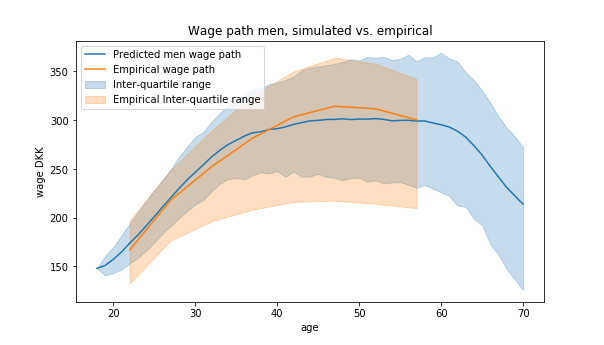
\includegraphics[width=1\linewidth]{figures/simulated_wage_path_variance_optimized_parameters_women.png}
  \caption{Men}
  \label{fig:sub1}
\end{subfigure}%
\begin{subfigure}{.5\textwidth}
  \centering
  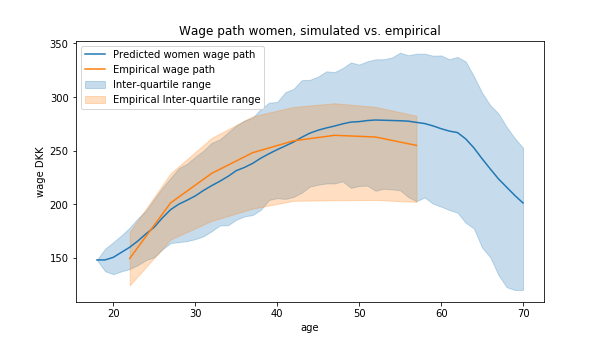
\includegraphics[width=1\linewidth]{figures/simulated_wage_path_variance_optimized_parameters_men.png}
  \caption{Women}
  \label{fig:sub2_wage_path}
\end{subfigure}
    \caption{Simulated Wage Process vs. Empirical Wage Process}
    \label{fig:sim_wage_vs_empirical_wage}
\end{figure}\label{sec:parameter_calibration}

Figure \ref{fig:sim_wage_vs_empirical_wage} compares the empirical wage process with the simulated. First looking to the \textit{wage path}, I conclude, that the Mincer equation seems to give a relatively good fit to the data even without taking education into account. The mean absolute error of the wage path of women is $10.61$ DKK, and for men the number is $5.84$ DKK, which considering the relatively simple parametric form of the process, is very good. Figure \ref{fig:sim_wage_vs_empirical_wage} also  show the empirical wage process is skewed. In this formulation of the mincer equation this is not possible. The width of the inter-quartile range seem to fit the wage path of men reasonably, but for women it slightly overshoots. I conclude the parameter values of the Mincer equation do seem to yield reasonable results, and they will be used throughout the paper. A side note about the empirical wage path of men and women is, that men do seem to experience a greater variance in their wage rates than women. Considering the work of both \textcite{francesconi_joint_2002} and \textcite{gayle_life-cyle_2006} that suggests that women on high income trajectories finds it less desirable to work, this is a puzzling result. The literature suggests that children could be one of the main drivers of heterogeneity observed in the wage rates of women, so when men have even higher wage rate differences, and these are not driven by children, one must conclude that other, probably equally important factors drive wage rate heterogeneity.



%\section{Deep Q-Function Iteration}

Deep Q-function iteration lends extends the classic value function iteration. However, value function iteration as discussed does not fare well in high dimensional state space and furthermore it's very computational heavy.

The idea is to approximate the integral by using a statistical method, and in this case Deep Learning (another machine learning method would be equally good). Still implore a backwards induction. Consider $f$ to be a machine learning function, that maps from State Space into $\vert \actionspace \vert$. I.e. For a given point in state space a prediction of the value function is computed for each possible action. This implies the method only is feasible for discrete state space. By trying to reduce the mean squared error between the the true values of the Q-function, and the prediction, the $\E[Q(a, s)]$ can be found, which corresponds to integration as could be done using f.x. Gauss Hermite or Monte Carlo integration.

\begin{algorithm}[H]
\SetAlgoLined
\KwResult{Write here the result }
 Initialize $\tilde{Age} = Age_{max}$\;
 Initialize empty lists for storing results: $X, Y$\;
 Initialize memory counter $j=1$\;
 \While{$\tilde{Age} > Age_{min}$}{
  Draw $\{s_i\}_{i=1}^{i=N}$, where $s_i \sim \statespace \mid Age=\tilde{Age}$ \;
  \ForEach{$s_i$}{
  Create empty array $Z$ of length $\mid \actionspace \mid$\;
  \eIf{$\tilde{Age}= Age_{max}$}{
   \ForEach{$a_k \in \actionspace$}{
    $Z[k] \leftarrow r(s_i, a_k)$ \;
   }
   }{
   \ForEach{$a_k \in \actionspace$}{
    $Z[k] \leftarrow r(s_i, a_k)$ + $\gamma \underset{a' \in \actionspace}{\max}\lsp \hat{q}(a', s_i') \rsp$\;
    }
  }
  $Y[j] \leftarrow Z, X[j] \leftarrow s_i$\;
  $j = j + 1$\;
  }
  Estimate $\hat{Q}$ by training a Deep NN using samples from $X, Y$.
 }
 \caption{Deep Q-function iteration solution method}
 \end{algorithm}

Since i use a deep neural network to approximate the $Q$-function, certain things need to be considered. First and foremost I need to consider the architecture of the network. Next I need to consider the train

For each age i draw 20.000 random samples. This is because any smaller number of draw seemed to be detrimental to the performance. This is inline with standard Deep Learning practices. These kinds of network is known to be very data hungry. When training the network i draw a random sample of 100.000 observations. If I have not yet accumulated 100.000 observations the algorithm draws all observations. The architecture of network is fairly simple being a two-layer fully connected network. First layer being 16 nodes wide, second fully connected layer being 8 nodes wide. I found that mini batching, did not seem to work well on this particular task, and instead i train on all observations, using a validation split of 30 \%, training for a maximum of 150 epochs and finally i allow for early stopping, that is, when the validation loss is not furthering decreasing i stop the training of the network. I do allow the algorithm a patience of 5. Implying that the algorithm will try to lower it's validation loss for five additional epochs before terminating the training.


\begin{figure}[ht]
\begin{subfigure}{.5\textwidth}
  \centering
  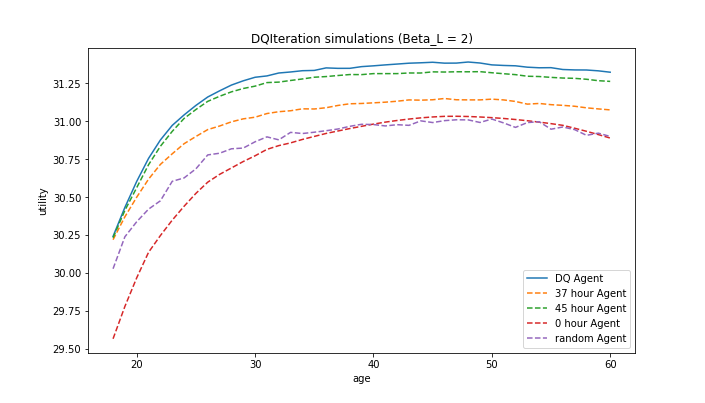
\includegraphics[width=1\linewidth]{figures/dqi_model1_beta_2_solution_benchmark_paths.png}
  \caption{Simulated Paths}
  \label{fig:dqi_solution_beta2_path}
\end{subfigure}%
\begin{subfigure}{.5\textwidth}
  \centering
  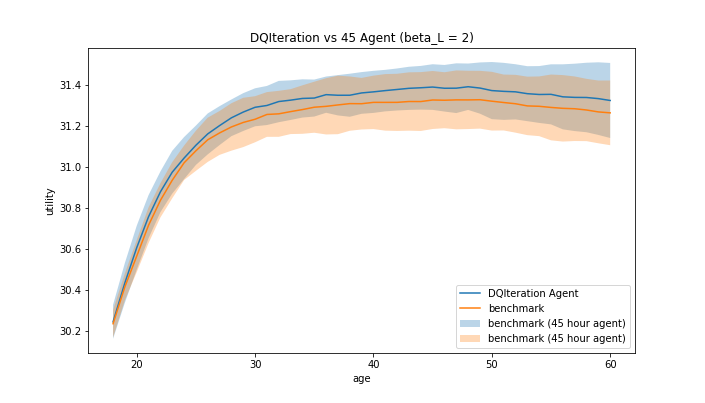
\includegraphics[width=1\linewidth]{figures/dqi_model1_beta_2_solution_benchmark_variance.png}
  \caption{Variance of Paths}
  \label{fig:dqi_solution_beta2_var}
\end{subfigure}
    \caption{Deep Q-iteration solution vs. benchmark $(\beta_L = 2)$}
    \label{fig:dqi_solution_beta2}
\end{figure}

\begin{figure}[ht]
\begin{subfigure}{.5\textwidth}
  \centering
  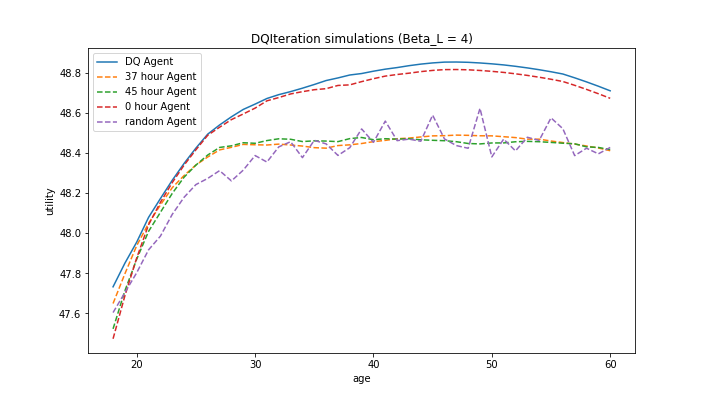
\includegraphics[width=1\linewidth]{figures/dqi_model1_beta_4_solution_benchmark_paths.png}
  \caption{Simulated Paths}
  \label{fig:dqi_solution_beta4_path}
\end{subfigure}%
\begin{subfigure}{.5\textwidth}
  \centering
  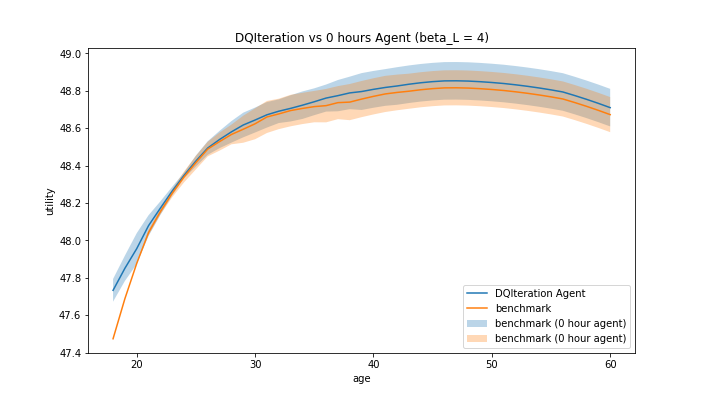
\includegraphics[width=1\linewidth]{figures/dqi_model1_beta_4_solution_benchmark_variance.png}
  \caption{Variance of simulations}
  \label{fig:dqi_solution_beta4_var}
\end{subfigure}
    \caption{Deep Q-iteration solution vs. benchmark $(\beta_L = 4)$}
    \label{fig:dqi_solution_beta4}
\end{figure}

%\section{Value Function Iteration solution}

As described in the section XXX, I first try to solve the model by Value Function iteration:

\begin{equation}
    \E_{t}[V_{t+1}(M_{t+1}, W_{t+1}, K_{t+1}, Q_{t+1})] = \int_{\epsilon_{t+1}} \int_{\gamma_{t+1}} \int_{\rho_{t+1}} V_{t+1} (M_{t+1}, W_{t+1}, K_{t+1}, Q_{t+1}) d\rho_{t+1} d \gamma_{t+1} d \epsilon_{t+1}
\end{equation}
%\section{Model (Extended)}

This will be where the extended model will be.

%\printbibliography
\end{document}
